% Chapter Template

\chapter{PHƯƠNG PHÁP THỰC HIỆN} % Main chapter title

\label{Chapter3} % Change X to a consecutive number; for referencing this chapter elsewhere, use \ref{ChapterX}

\section*{Tóm tắt chương}
Ở chương này, chúng tôi sẽ trình bày chi tiết kiến trúc và cách hoạt động của mô hình \textbf{XFedHunter}, gồm hai thành phần là mô hình học liên kết cho các hệ thống phát hiện tấn công APT và mô hình săn tìm tấn công APT. Trong đó, mô hình học liên kết cho các hệ thống phát hiện tấn công APT sẽ mô tả cách các đối tác tham gia huấn luyện các hệ thống IDS và mô hình săn tìm tấn công APT sẽ mô tả kiến trúc và cách vận hành của các thành phần bảo mật được đề xuất ở mỗi đối tác.

\section{Mô hình học liên kết cho các hệ thống phát hiện tấn công APT} \label{sec:FL-model}

Nhằm giải quyết quyết vấn đề dữ liệu cho hệ thống phát hiện tấn công APT, chúng tôi đã đưa ra mô hình học liên kết sử dụng thuật toán FedAvg \cite{mcmahan2017communication} để huấn luyện các hệ thống IDS sử dụng học sâu của các tổ chức tham gia vào quá trình liên kết như trong \textbf{Hình \ref{fig:proposed-FL-model}}.

\begin{figure}[ht]
	\centering
	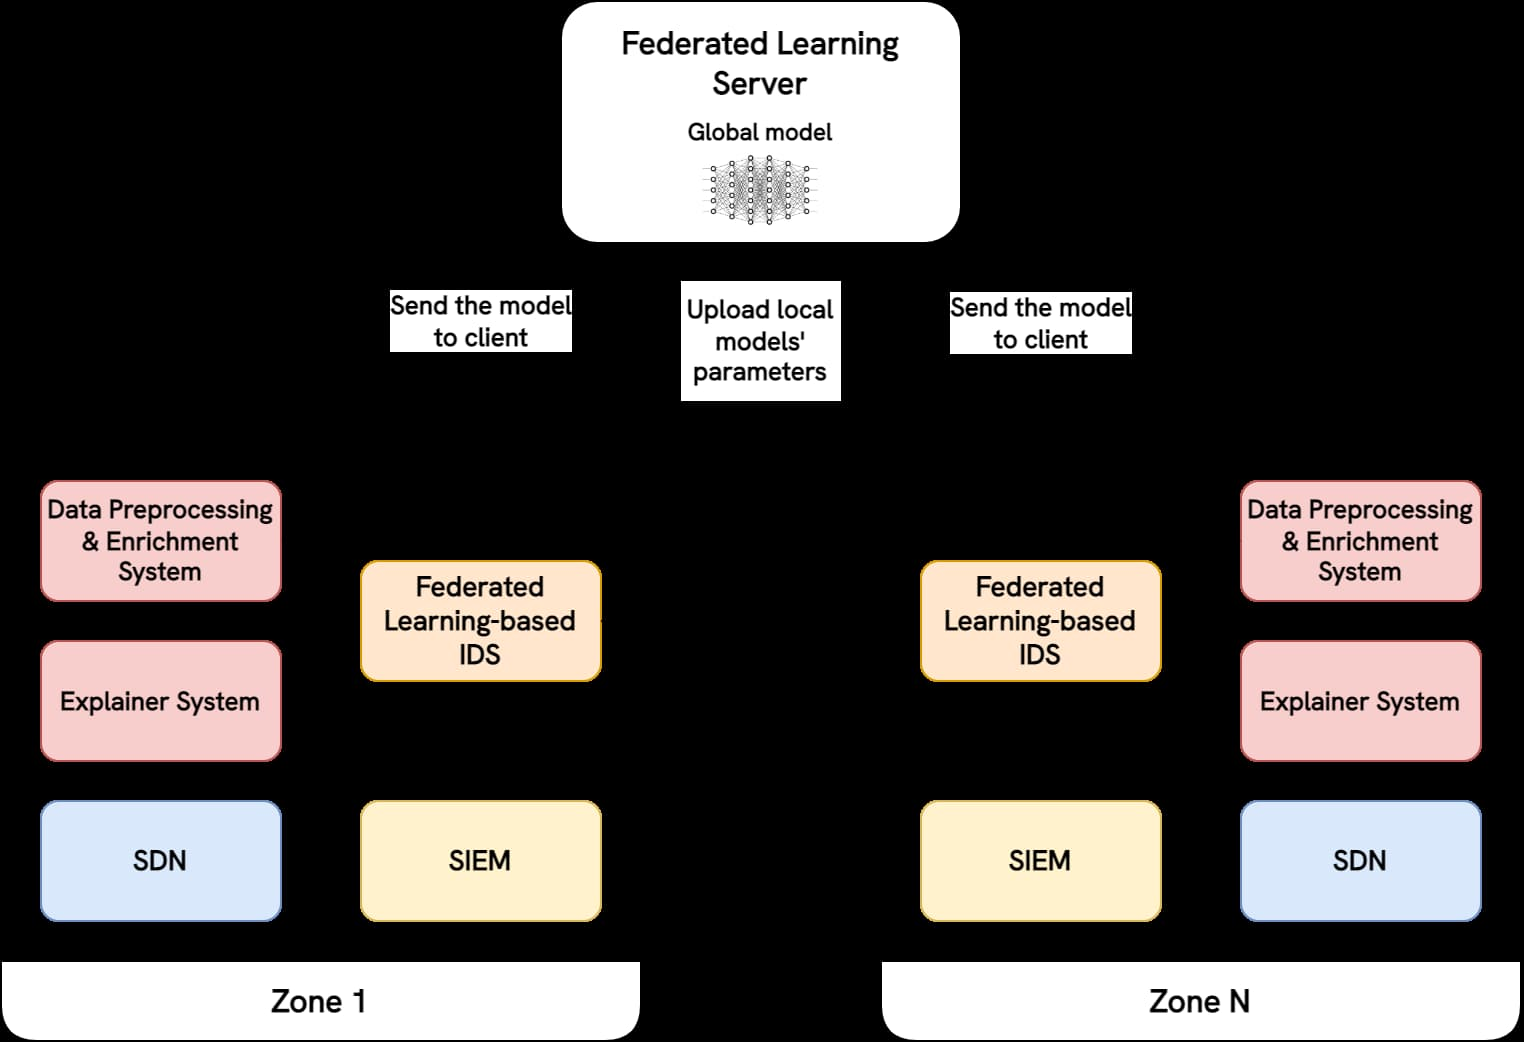
\includegraphics[width=\textwidth]{src/images/chapter3/proposed-model.jpg}
	\caption{Mô hình học liên kết cho các hệ thống phát hiện tấn công APT}
	\label{fig:proposed-FL-model}
\end{figure}

\bigbreak\noindent
Trong mô hình được đề xuất, từng tổ chức tham gia vào quá trình huấn luyện liên kết được xem như một vùng (zone). Trong mỗi vùng, hệ thống IDS sẽ đóng vai trò giao tiếp trực tiếp với máy chủ trung tâm để nhận và gửi các tham số huấn luyện cũng như là nơi thực hiện quá trình huấn luyện cục bộ. Cụ thể, ở mọi vòng huấn luyện, các tổ chức tham gia và máy chủ trung tâm sẽ thực hiện các bước sau:

\begin{itemize}
    \item Đầu tiên, hệ thống IDS ở mỗi vùng sẽ giao tiếp với máy chủ trung tâm để nhận các tham số huấn luyện. Trong thuật toán học liên kết được chúng tôi sử dụng, máy chủ trung sẽ gửi các trọng số của mô hình toàn cục cho các đối tác.
	
    \item Tiếp theo, các tổ chức tham gia sẽ thực hiện huấn luyện các mô hình cục bộ bằng tham số được gửi từ máy chủ trung tâm bằng dữ liệu riêng của tổ chức.
	
    \item Sau khi quá trình huấn luyện cục bộ kết thúc, các đối tác sẽ gửi các tham số được huấn luyện cục bộ lại cho máy chủ trung tâm. Trong đó, các tham số được huấn luyện cục bộ sẽ là các trọng số của mô hình vừa được huấn luyện xong tại các tổ chức tham gia và cống hiến của tổ chức đó (thường là kích thước dữ liệu được dùng để huấn luyện mô hình cục bộ).
	
    \item Sau khi nhận được đầy đủ các tham số huấn luyện cục bộ, máy chủ trung tâm sẽ tiến hành tổng hợp các tham số huấn luyện mới dựa trên \textbf{Công thức \ref{eq:agg_fedavg}}.
	
    \item Cuối cùng, máy chủ trung tâm sẽ gửi các tham số huấn luyện mới được tạo ra đến các đối tác để tiếp tục huấn luyện hoặc sử dụng để tạo ra các hệ thống IDS sử dụng trong phát hiện tấn công APT.
\end{itemize}

\bigbreak\noindent
Trong thuật toán FedAvg, các tham số huấn luyện cục bộ được tổng hợp ở máy chủ trung tâm theo công thức sau:
\begin{equation}
    w = \sum_{k=1}^{K} \frac{n_k}{n} w_k
    \label{eq:agg_fedavg}
\end{equation}

\bigbreak\noindent
Trong đó, $w$ là các trọng số mới của mô hình toàn cục, $K$ là các tổ chức tham gia vào quá trình huấn luyện, $w_k$ là các trọng số của mô hình cục bộ được huấn luyện bởi tổ chức thứ $k$, $n_k$ là kích thước của dữ liệu được dùng để huấn luyện mô hình cục bộ của tổ chức thứ $k$, và $n$ tổng kích thước dữ liệu dùng để huấn luyện của tất cả các đối tác.


%Từ quá trình huấn luyện cộng tác không ngừng trên, các hệ thống IDS của các vùng sẽ có khả năng nhận diện các mối đe dọa trong hệ thống đồng thời đảm bảo tính riêng tư của dữ liệu của các bên tham gia cũng như nâng cao khả năng phát hiện các 0-day attack thông qua việc sử dụng dữ liệu từ nhiều môi trường khác nhau. Hơn thế nữa, để nâng cao khả năng ứng dụng của hệ thống IDS trong các giải pháp săn tìm mối đe dọa của trung tâm SOC, hệ thống làm giàu thông tin được triển khai và kết hợp với các giải pháp bảo mật hiện có như hệ thống quản lý log Và sự kiện tập trung (Security information and event management - SIEM), thông tin mối đe dọa an ninh mạng (Cyber threat intelligence - CTI), ... nhằm nhân cao hơn nữa tính khả dụng cũng như hiệu quả của giải pháp trong môi trường thực tế.


\section{Mô hình săn tìm tấn công APT}

Mô hình săn tìm tấn công APT được đề xuất gồm có sáu phần chính: mạng SDN, hệ thống SIEM, hệ thống IDS, hệ thống tiền xử lý và làm giàu thông tin (hệ thống DPE), hệ thống CTI, và Hệ thống diễn giải dự đoán. Mô hình đề xuất chi tiết được trình bày trong \textbf{Hình \ref{fig:proposed-APT-hunting-model}}.

\begin{figure}[ht]
	\centering
	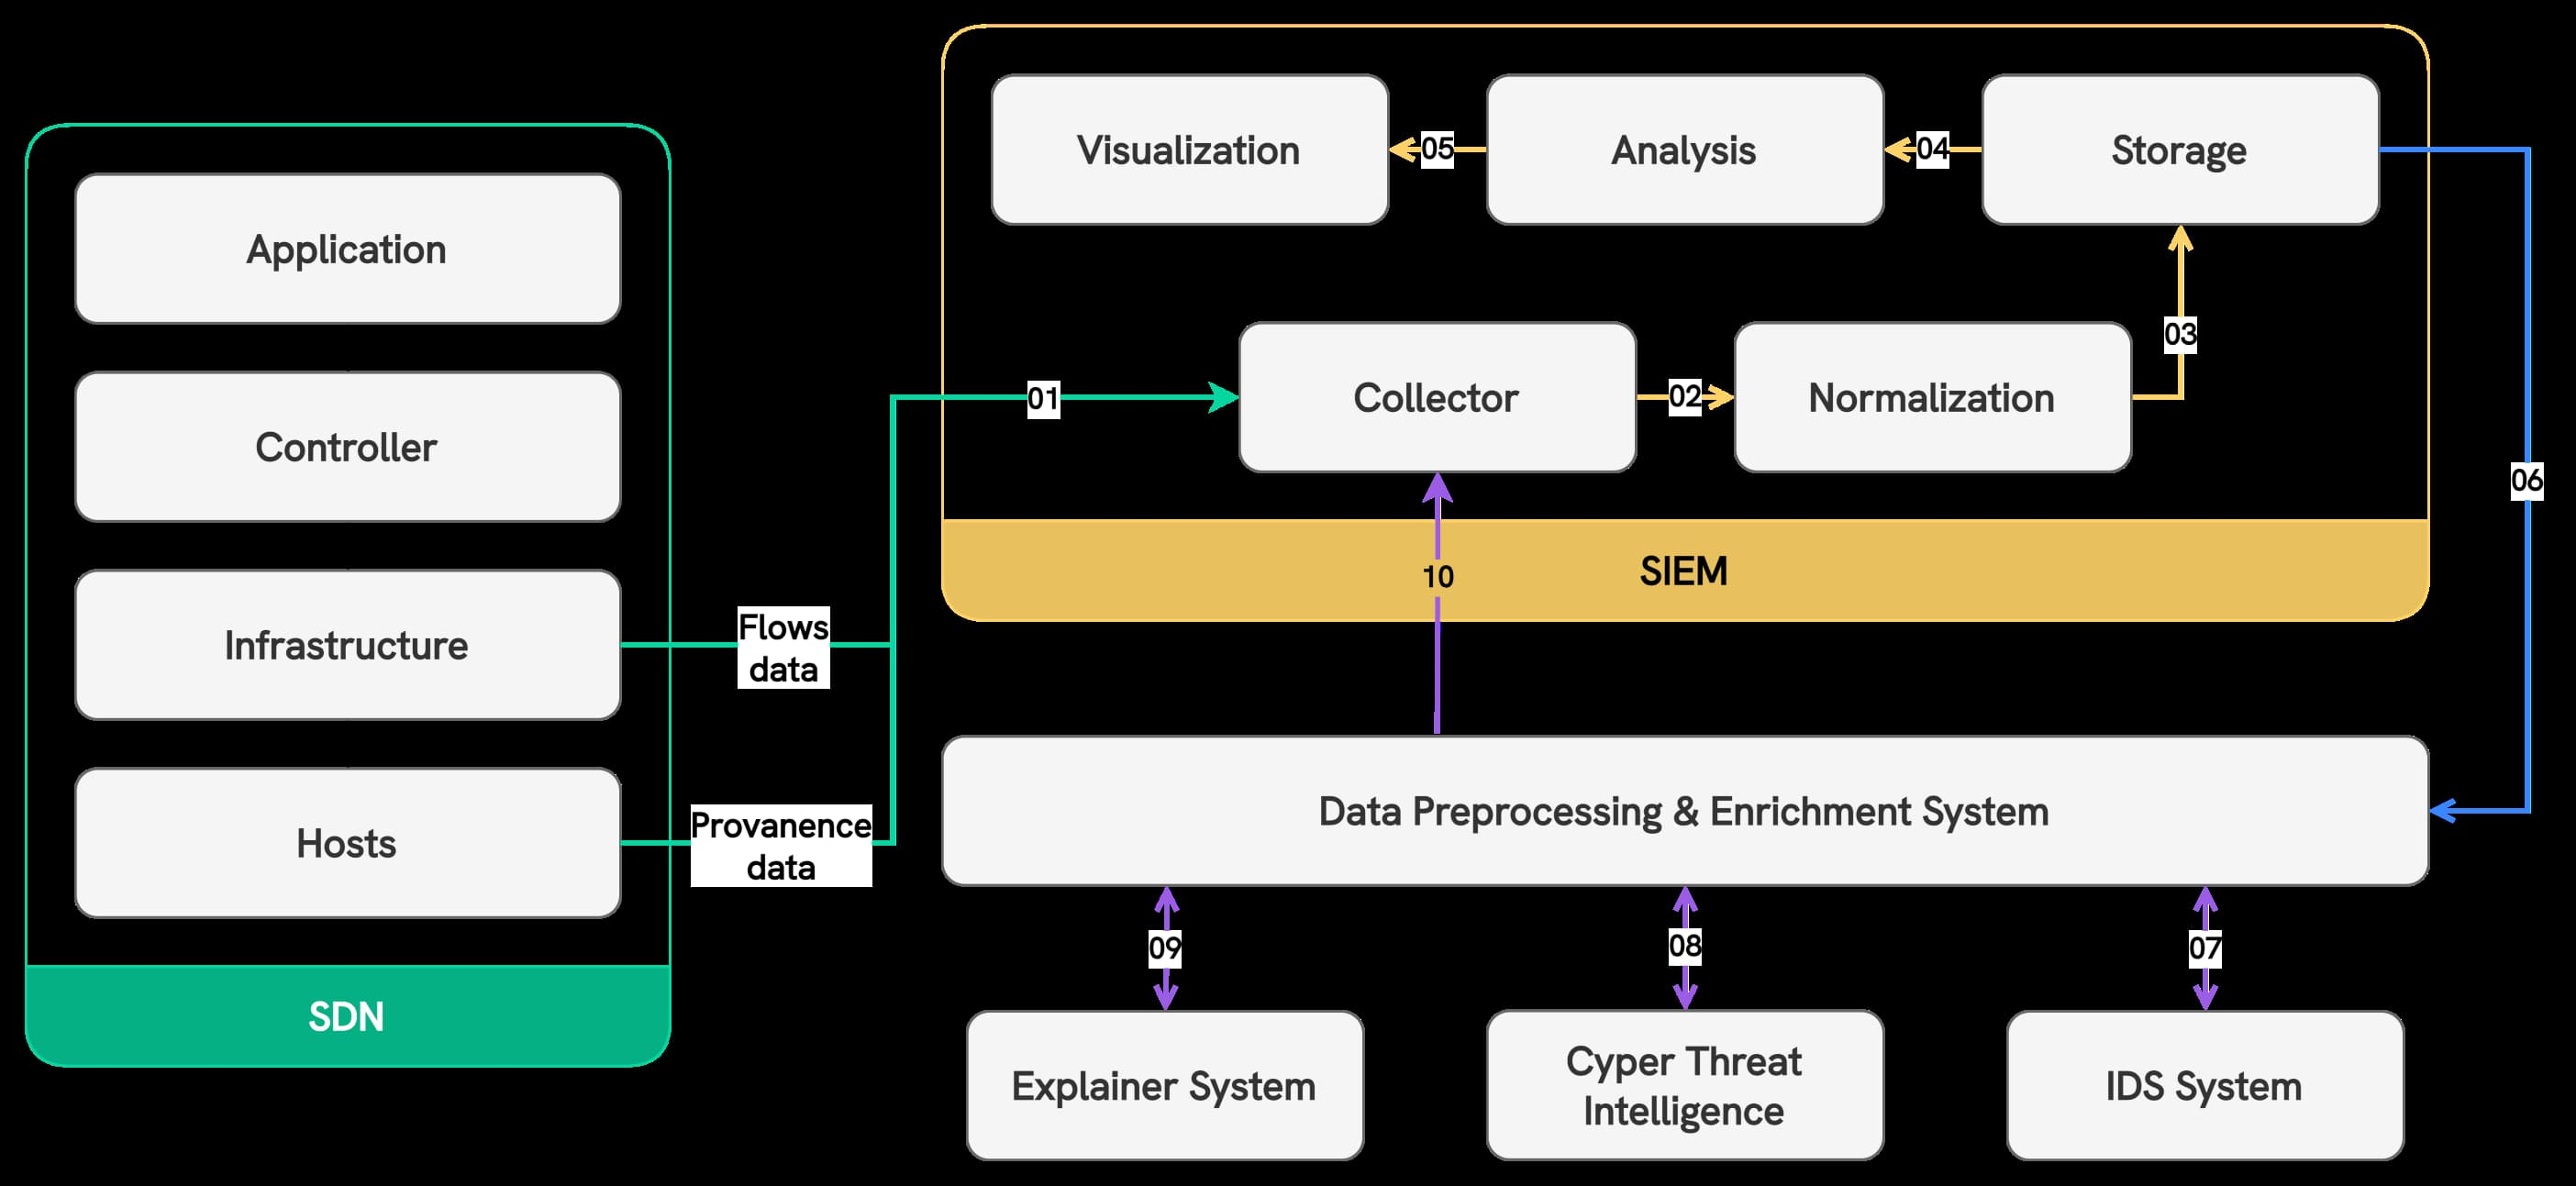
\includegraphics[width=\textwidth]{src/images/chapter3/zone-model.jpg}
	\caption{Mô hình săn tìm tấn công APT}
	\label{fig:proposed-APT-hunting-model}
\end{figure}

\bigbreak\noindent
Trong mô hình đề xuất, dữ liệu được thu thập từ các switch và các host trong mạng SDN sẽ được thu thập bởi bộ thu thập của SIEM (SIEM collector). Tiếp đến, hệ thống SIEM sẽ chuẩn hóa và lưu trữ dữ liệu được thu thập. Dữ liệu chuẩn hóa được lưu trữ tiếp đến sẽ được hệ thống DPE sử dụng để phát hiện tấn công APT bằng cách xử lý và gửi các dữ liệu cần được phân tích đến hệ thống IDS. Bên cạnh đó, nhằm hỗ trợ các nhà săn tìm trong quá trình truy vết cuộc tấn công cũng như quá trình xác định độ tin cậy của dự đoán đến từ hệ thống IDS, hệ thống DPE sẽ gửi các thông tin cần thiết đến hệ thống CTI và hệ thống diễn giải dự đoán để thu được các thông tin làm giàu. Các thông tin làm giàu thường bao gồm thông tin trả về từ hệ thống CTI, hệ thống diễn giải dự đoán và một số dữ liệu khác được trích xuất bởi hệ thống DPE từ dữ liệu đầu vào. Cuối cùng, kết quả dự đoán từ hệ thống IDS sẽ được kết hợp với thông tin làm giàu và được lưu lại dưới dạng \textit{log} trong hệ thống DPE. \textit{Log} này sẽ được thu thập bởi hệ thống SIEM, sau đó được lưu trữ và chờ được sử dụng.

 %nếu kết quả trả về từ hệ thống IDS xác định dữ liệu đầu vào chứa hoạt động bất thường  hệ thống PDE cũng sẽ thực hiện truy xuất thêm các thông tin từ hệ thống CTI

%Sau khi thông tin từ nơi lưu trữ được chuyển đến hệ thống tiền xử lý và làm giàu thông tin, các thuộc tính cần thiết cho quá trình huấn luyện các thuật học sâu sẽ được trích xuất và gửi đến hệ thống IDS. Đồng thời, trong quá trình trích xuất thuộc tính từ dữ liệu đầu vào thì hệ thống sẽ thực hiện trích xuất các thông tin làm giàu. Sau đó, các thông tin làm giàu này sẽ được kết hợp với dữ liệu từ hệ thống OpenCTI nhằm mục đích tăng thêm độ đậm đặc của thông tin. Cuối cùng, kết quả dự đoán từ hệ thống IDS sẽ được kết hợp với thông tin làm giàu và được lưu lại dưới dạng \textit{log}. Sau đó, \textit{log} này sẽ được gửi đến hệ thống SIEM để chờ được phân tích và sử dụng.

\subsection{Mạng SDN}
Trong kiến trúc đề xuất, chúng tôi xác định rằng các hoạt động, sự kiện đến từ một cuộc tấn công APT sẽ tồn tại trong mạng SDN dưới dạng các \textit{flow} chạy qua các SDN switch và các dữ liệu \textit{log} tồn tại tại các điểm đầu cuối. Các dữ liệu này cần được thu thập và đưa đến SIEM để tiến hành lưu trữ và phân tích. Để có thể tận dụng được triệt để được các nguồn dữ liệu trên, chúng tôi đã cấu hình các switch cốt lõi (các switch mà hầu hết các lưu lượng mạng phải đi qua để tra bên ngoài cũng như di chuyển giữa các vùng mạng) gửi các \textit{flow} mà các switch này bắt được thông qua giao thức NetFlow đến SIEM collector. Đối với dữ liệu \textit{log} trên các điểm đầu cuối, chúng tôi sử dụng SIEM agent (phần mềm thường được tích hợp sẵn trong các hệ thống SIEM hiện hành để thu thập dữ liệu trên các thiết bị đã được cài đặt phần mềm).

\subsection{Hệ thống SIEM}
Các dữ liệu sau khi được thu thập từ mạng SDN sẽ được xử lý, chuẩn hóa một cách phù cho việc lưu trữ và sử dụng. Bên cạnh đó, hệ thống SIEM cũng đảm nhận vai trò thu thập các kết quả dự đoán bất thường đã được làm giàu bởi hệ thống DPE. Cuối cùng, các dữ liệu được thu thập sẽ được sử dụng trong phân tích và điều tra về các hoạt động bất thường trong hệ thống. Nhờ vào khả năng cho phép các nhà săn tìm có thể truy xuất các sự kiện, thông tin và các kết quả phân tích bất thường từ toàn mạng theo thời gian thực, hệ thống SIEM là một thành phần không thể thiếu trong quá trình triển khai các giải pháp săn tìm chủ động. Bởi vì, các giải pháp săn tìm này đòi hỏi phải truy cập một lượng lớn thông tin tại nhiều nơi trong hệ thống để có thể phát hiện và truy vết một cách triệt để các cuộc tấn công phức APT phức tạp, như đã được thể hiện qua nhiều nghiên cứu \cite{caltagirone2013diamond}, \cite{gunter2018practical}, \cite{ajmal2021offensive}, \cite{jadidi2021threat}. Ngoài ra, trong kiến trúc đề xuất, hệ thống SIEM được kết hợp với hệ thống DPE để tạo ra một chu trình kín, góp phần tự động hóa các quá trình phân tích thủ công tốn kém. Từ đó, rút ngắn thời gian phát hiện, phân tích và ngăn chặn các cuộc tấn công APT.

\subsection{Hệ thống IDS}
Nhằm tạo ra một hệ thống phát hiện toàn diện và hiệu quả trong việc phân tích các sự kiện có thể dẫn đến một cuộc tấn công APT, chúng tôi quyết định triển khai kết hợp hai hệ thống IDS sử dụng nơ-ron nhân tạo là NIDS và PIDS. Cụ thể, chúng tôi đã sử dụng một mô hình học sâu được gọi là GRU\&CNN cho NIDS. Mô hình này sử dụng kết hợp hai mạng nơ-ron là CNN và GRU được cải tiến dựa trên mô hình DeepFed để có thể dự đoán được hoạt động bất thường trong mạng SDN, thông qua việc phân tích dữ liệu mạng tồn tại dưới định dạng NetFlow.

\bigbreak\noindent
Kiến trúc đề xuất của mô hình GRU\&CNN được miêu tả như trong \textbf{Hình \ref{fig:GRU&CNN-model}}. Trong kiến trúc trên, đầu vào $x$ (gồm các thuộc tính từ $x_1$ đến $x_n$) được đưa lần lượt vào GRU mô-đun và CNN mô-đun để trích xuất các khuôn mẫu dữ liệu tiềm năng. Trong đó, GRU mô-đun sẽ phụ trách học các khuôn mẫu dữ liệu ẩn từ các thuộc tính có tính liên tục (IP nguồn-đích, port nguồn-đích, thời lượng kết nối, số bytes tin gửi và nhận, ...). Trong khi đó, CNN mô-đun sẽ phụ trách học các khuôn mẫu dữ liệu ẩn từ các thuộc tính có tính rời rạc (loại giao thức ở các tầng như ARP, ICMP, TCP, UDP, DNS, HTTP,... và các thuộc tính của gói tin). Sau đó, các thuộc tính ẩn quan trọng từ các khuôn mẫu dữ liệu ẩn được trích xuất bởi CNN mô-đun thông qua lớp lớp gộp cực đại toàn cục. Tiếp đến, các khuôn mẫu dữ liệu ẩn được tạo ra bởi hai mô-đun (lần lượt là $v$ và $\mu$) sẽ được nối lại và đưa vào MLP (Multi-layer Perceptron) mô-đun. Cuối cùng, MLP mô-đun sẽ tổng hợp các thông tin từ hai dữ liệu ẩn trên và đưa ra dự đoán về \textit{flow} được phân tích có phải là bất thường hay không dưới dạng giá trị từ $0$ đến $1$.

\begin{figure}[ht]
	\centering
	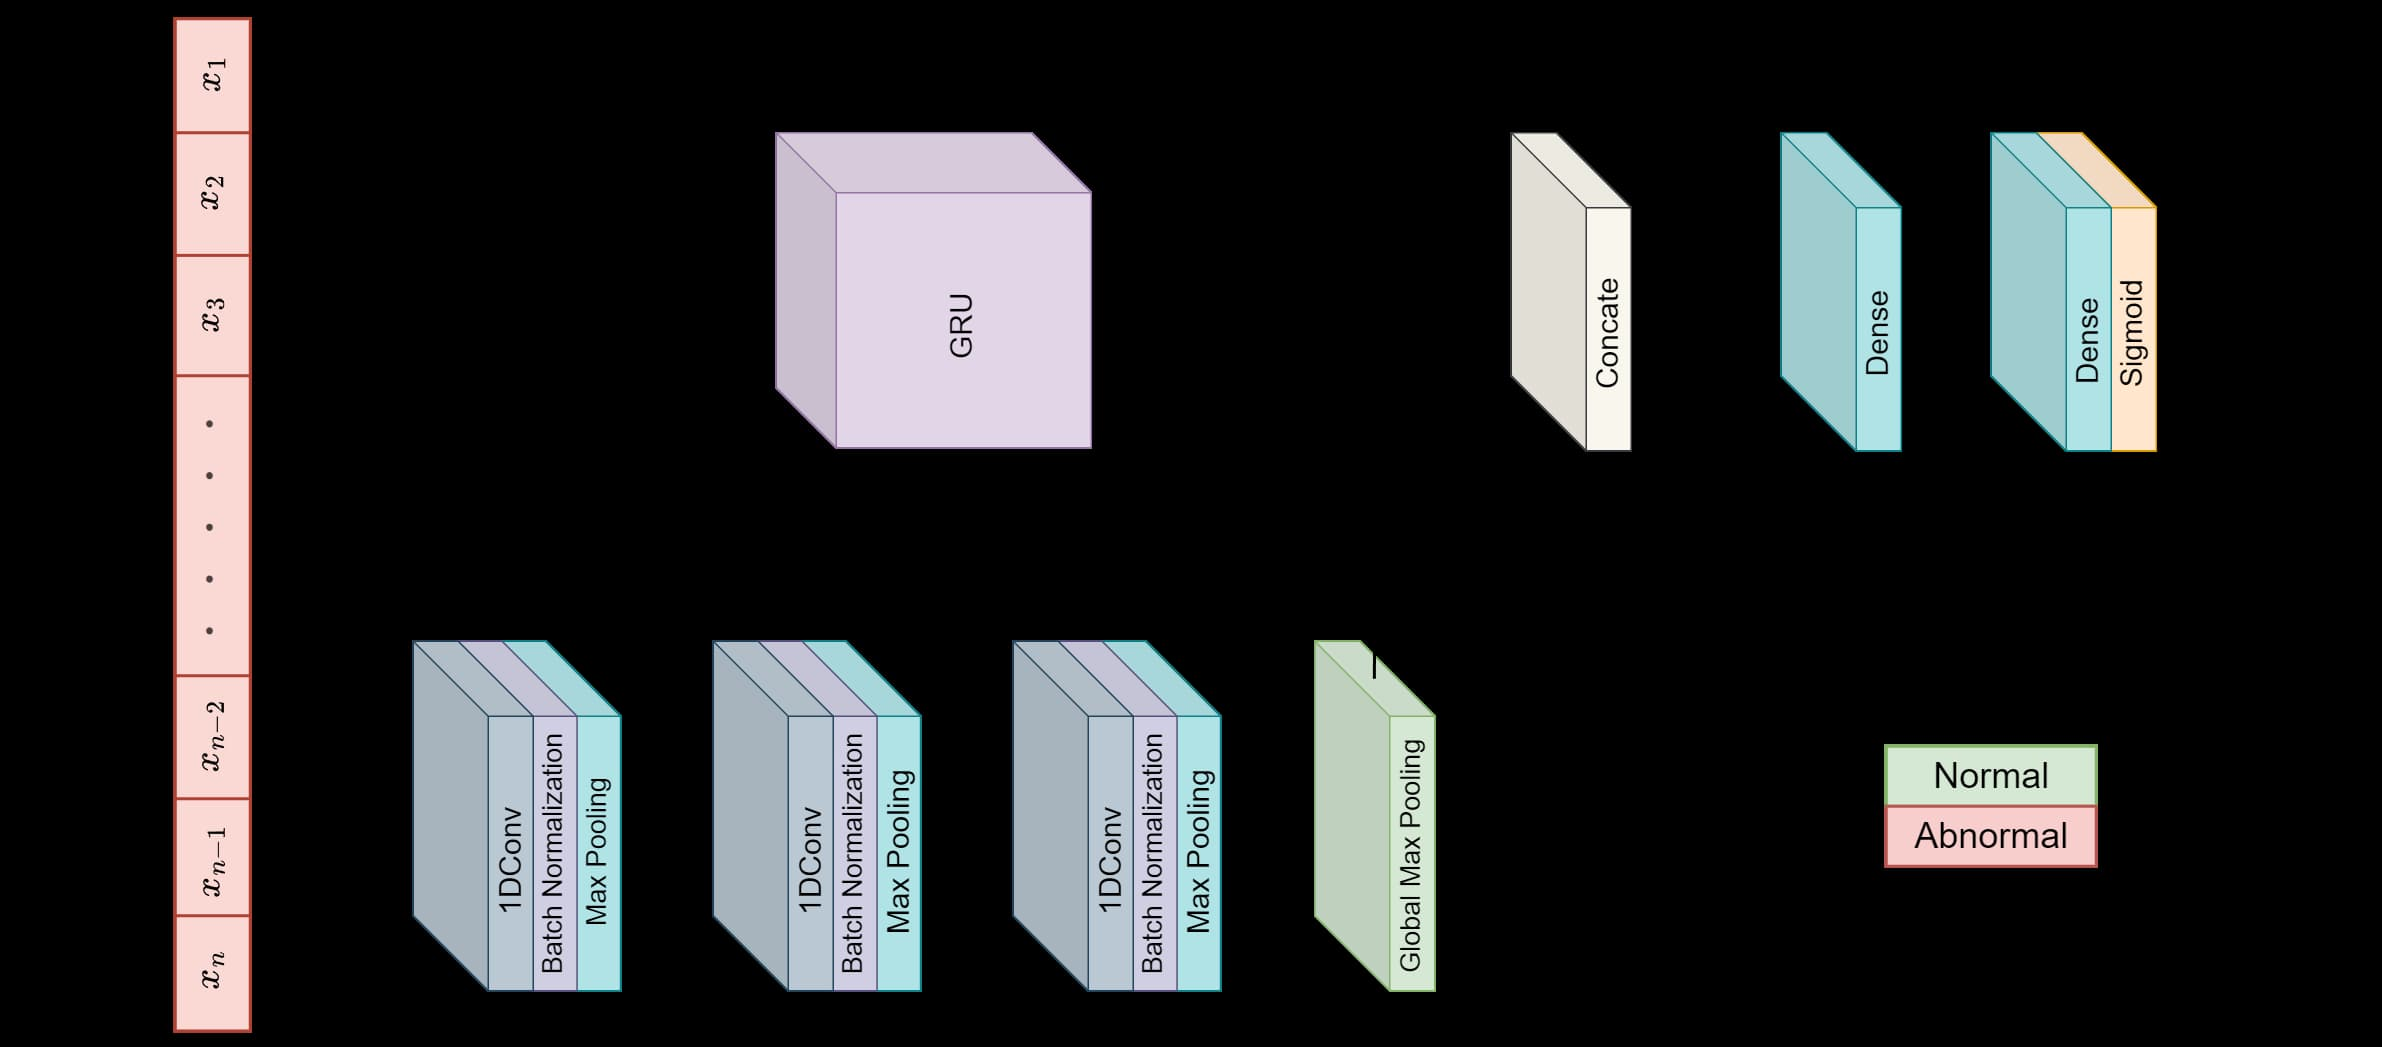
\includegraphics[width=\textwidth]{src/images/chapter3/GRU&CNN.jpg}
	\caption{Mô hình GRU\&CNN được đề xuất cho NIDS}
	\label{fig:GRU&CNN-model}
\end{figure}

\bigbreak\noindent
Đối với PIDS, chúng tôi sử dụng mô hình GraphSAGE tích hợp Transformer được gọi tắt là TGraphSAGE để phân tích đồ thị được tạo bởi dữ liệu \textit{log} được thu thập bởi hệ thống SIEM. Mô hình kết hợp được đề xuất có khả năng phát hiện các chuỗi sự kiện bất thường có thể gây ra một cuộc tấn công APT ở các điểm đầu cuối và có kiến trúc như \textbf{Hình \ref{fig:GraphSAGE-model}}. Đầu tiên, các \textit{log} được thu thập bởi hệ thống SIEM được chuyển thành đồ thị nguồn gốc $G$. Tuy nhiên, các thuộc tính giữa các nút hoặc giữa các cạnh trên đồ thị thường không đồng nhất (khác số lượng thuộc tính) và khó xử lý (các thuộc tính tồn tại ở nhiều loại và có phạm vi giá trị gần như vô hạn). Ngoài ra, mô hình GraphSAGE truyền thống chỉ có thể học dựa trên thuộc tính của nút và bỏ phí các thông tin quan trọng từ các cạnh. Để giải quyết vấn đề trên, mô hình Transformer được đưa vào để đồng nhất các thuộc tính trên các nút và đưa các thuộc tính của các cạnh vào trong các nút để tạo thành đồ thị nhúng $G'$. Đồ thị mới được tạo thành chỉ gồm các thuộc tính đồng nhất (bằng nhau về số lượng thuộc tính giữa các nút) và dễ xử lý (thuộc tính là các số thực có thể dễ dàng được học bởi các nơ-ron nhân tạo) của các nút. Sau đó, mô hình GraphSAGE sẽ phân tích và phát hiện các nút bất thường trên đồ thị $G'$.

\begin{figure}[ht]
	\centering
	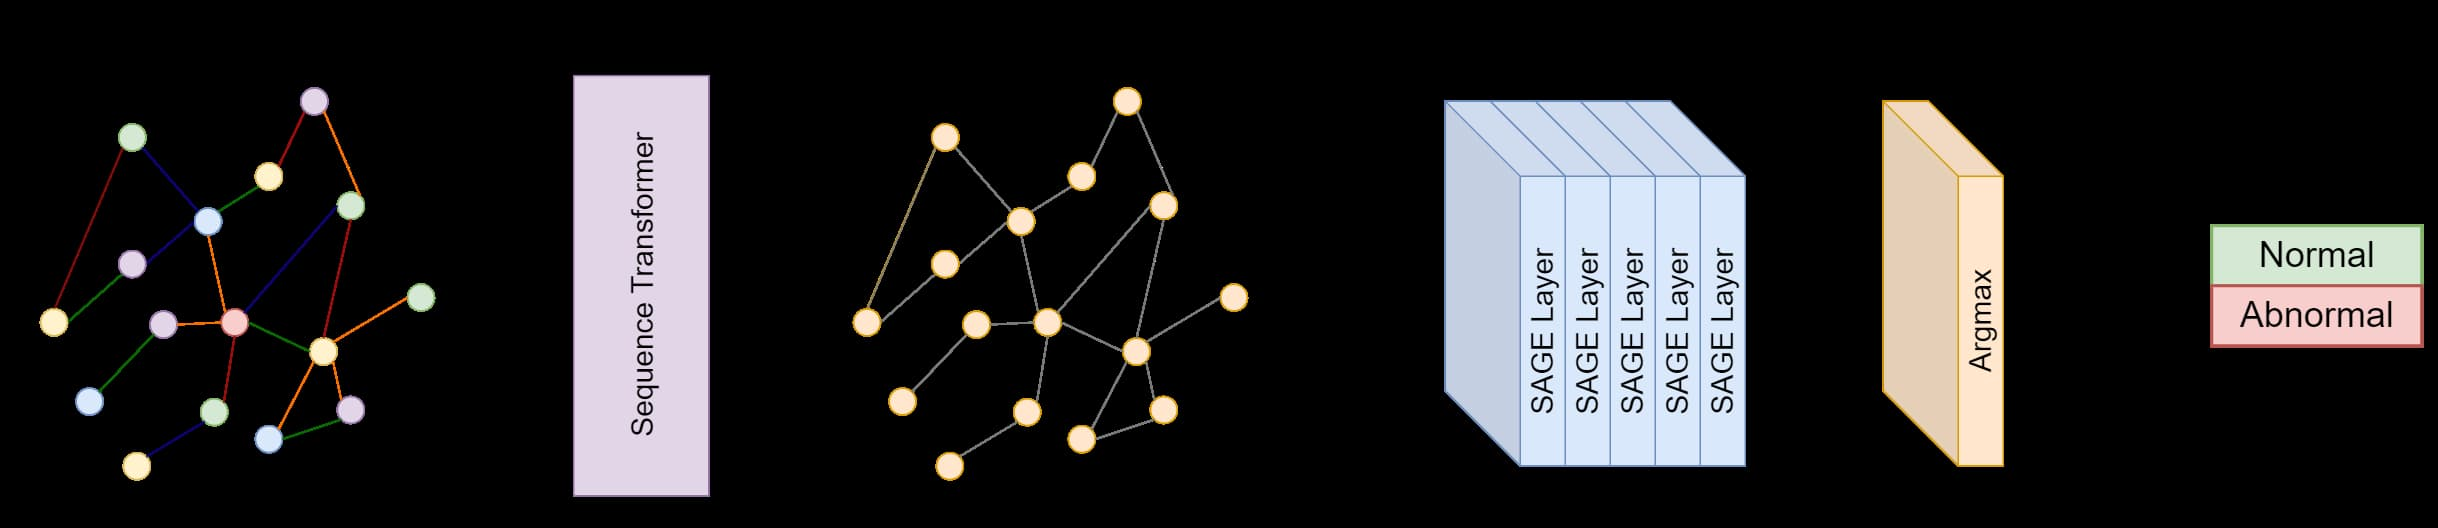
\includegraphics[width=\textwidth]{src/images/chapter3/GraphSAGE.jpg}
	\caption{Mô hình TGraphSAGE được đề xuất cho PIDS}
	\label{fig:GraphSAGE-model}
\end{figure}

\bigbreak\noindent
Ngoài ra, cả hai mô hình GRU\&CNN và TGraphSAGE đều được gia tăng hiệu suất thông qua việc huấn luyện bằng phương pháp học liên kết như đã được đề cập trong \textbf{Mục \ref{sec:FL-model}}.

\subsection{Hệ thống CTI}
Việc phát triển các phương pháp, kỹ thuật, công cụ tấn công và các mã độc mới trong các cuộc tấn công APT là rất tốn kém nên các kẻ tấn công thường có xu hướng sử dụng lại một phần hoặc dựa hoàn toàn trên các phương pháp và công cụ sẵn có. Nắm bắt được xu hướng đó, chúng tôi đã tích hợp hệ thống CTI vào kiến trúc đề xuất. Với nguồn dữ liệu đa dạng về các cuộc tấn công APT được thu thập và chia sẻ thông qua hệ thống CTI, các nhà săn tìm có thể dễ dàng đối chiếu các dấu hiệu bất thường, các sự kiện tình nghi là tấn công APT với các thông tin được ghi nhận từ các cuộc tấn công đã xảy ra trước đây cũng như các dấu hiệu và sự kiện gây ra bởi các kỹ thuật, phương pháp tấn công mới được phát hiện và chưa được phổ biến. Với sự tham gia của hệ thống CTI, chúng ta có thể đẩy nhanh quá trình phát hiện và phân tích các cuộc tấn công APT cũng như hỗ trợ cho quá trình xác thực tính đúng đắn của các quyết định đến từ hệ thống IDS.

\subsection{Hệ thống diễn giải dự đoán}
Hệ thống diễn giải dự đoán được xây dựng dựa trên các phương pháp học máy khả giải cần đại để xác định các nhân tố quan trọng ảnh hưởng đến quyết định của các hệ thống IDS. Từ đó, hỗ trợ cho các nhà săn tìm trong việc xác minh tính đúng đắn của các dự đoán từ các hệ thống IDS cũng như hỗ trợ cho quá trình phân tích các cuộc tấn công APT. Do tính chất khác nhau về dữ liệu đầu vào của NIDS và PIDS được đề xuất (NIDS dựa trên các thuộc tính trích xuất từ các \textit{flow} dưới định dạng NetFlow, PIDS dựa trên đồ thị được tạo thành từ \textit{log} của các điểm đầu cuối) nên phương pháp học máy khả giải cho hai hệ thống IDS cũng có phần khác biệt. Cụ thể, chúng ta sẽ sử dụng KernelSHAP từ bộ khung SHAP để xác định các thuộc tính quan trọng có ảnh hưởng lớn đến các quyết định của NIDS. Đối với PIDS, chúng sẽ sử dụng GNNExplainer để xác định một đồ thị con từ đồ thị gốc với các cạnh có ảnh hưởng đáng kể đến dự đoán của hệ thống. Ngoài ra, chúng tôi còn cung cấp thêm một phương pháp để kiểm tra độ tin cậy của các dự đoán từ các mô hình IDS. Kiến trúc tổng quan của hệ thống diễn giải dự đoán được mô tả như \textbf{Hình \ref{fig:explainer-module}}.

\begin{figure}[ht]
	\centering
	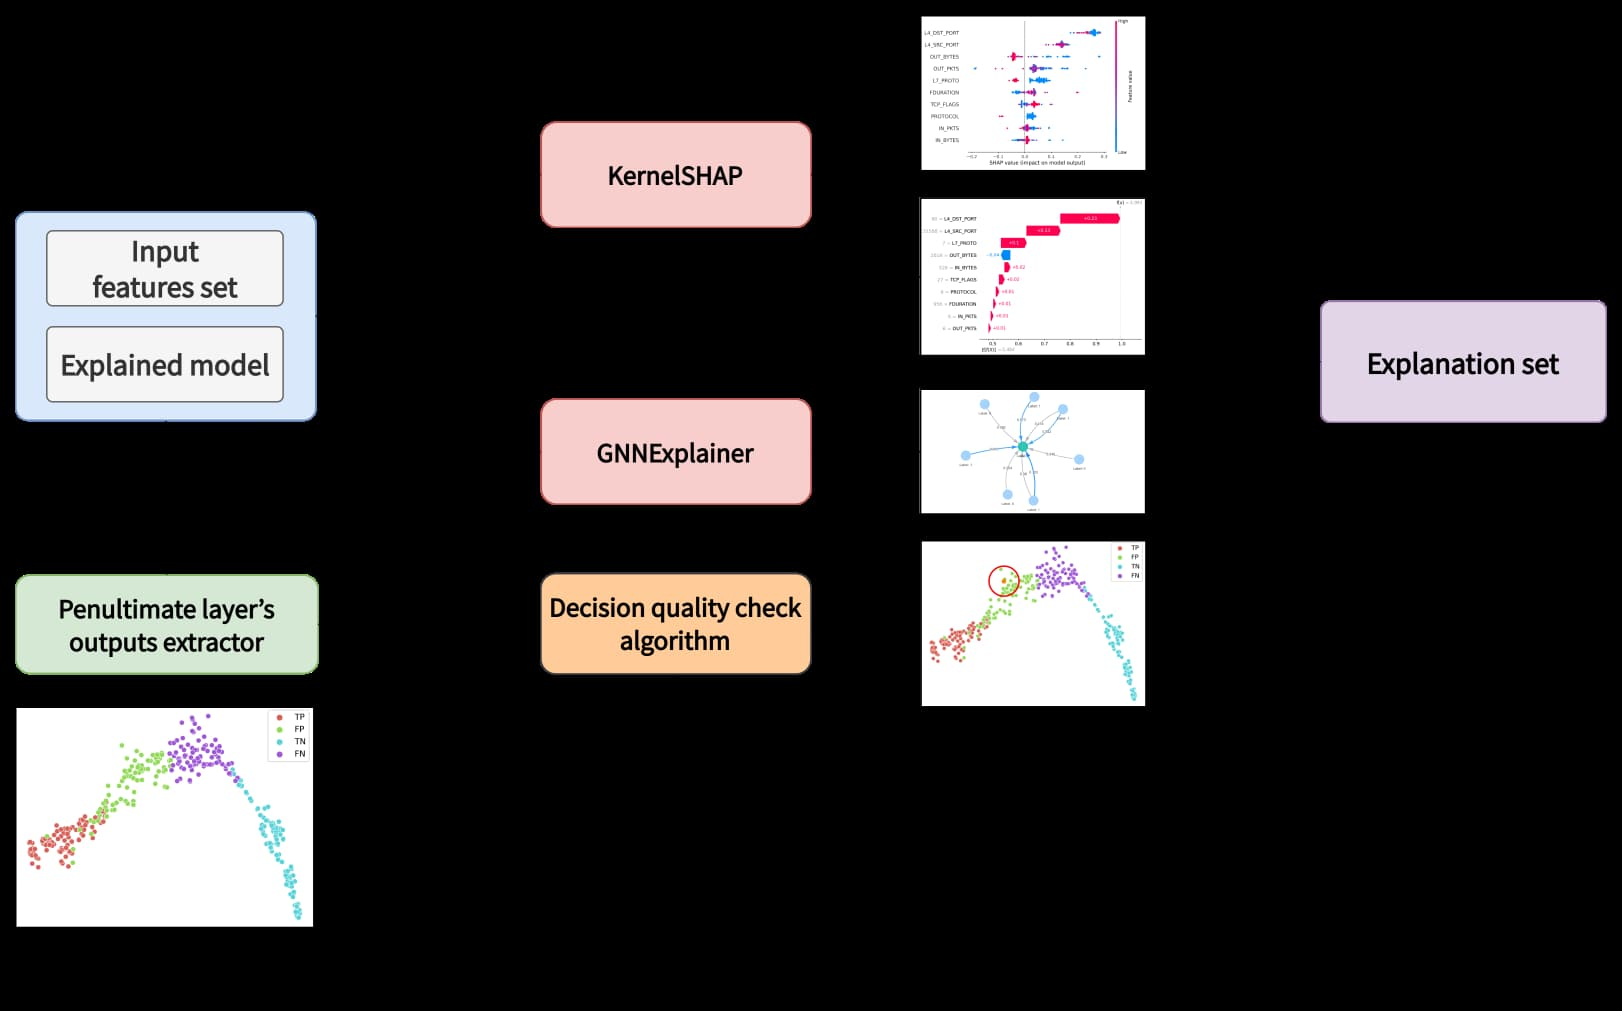
\includegraphics[width=\textwidth]{src/images/chapter3/explainer-module.jpg}
	\caption{Kiến trúc được đề xuất cho hệ thống diễn giải dự đoán}
	\label{fig:explainer-module}
\end{figure}

\subsubsection{Phương pháp diễn giải dự đoán của NIDS}
Bộ khung SHAP tính toán độ ảnh hưởng của các thuộc tính đến một dự đoán của NIDS thông qua việc tính toán giá trị Shapley của các thuộc tính đó. Cụ thể, một giải thích tạo bộ khung SHAP cho một dự đoán được thực hiện bởi mô hình $f$ cho một đầu vào $x$ có $M$ thuộc tính có thể được xác định thông qua hàm $g$ như sau:
\begin{equation} \label{eq:SHAP_explain_function}
    g(z') = \varphi_0 + \sum_{j=1}^{M} \varphi_j z'_j
\end{equation}
Trong đó, giá trị Shapley của $\varphi_j$ đại diện cho đóng góp của đặc trưng thứ $j$ trong $x$, $z'$ là một vectơ nhị phân biểu diễn một tập các thuộc tính được đơn giản hóa của $x$ ($z' \in {0, 1}^M$). Các phần tử trong $z'$ xác định rằng $\varphi_j$ nào nên được đưa vào giải thích và $\varphi_j$ nào sẽ không được đưa vào (1 là sẽ có mặt trong giải thích và 0 là sẽ không có mặt trong giải thích). Cuối cùng, $\varphi_0$ đại diện cho đầu ra của mô hình khi tắt tất cả các đầu vào đơn giản hóa (tức là tất cả các giá trị trong $z'$ được đánh dấu là 0).

\bigbreak\noindent
Trong \textbf{Công thức \ref{eq:SHAP_explain_function}}, Giá trị của $\varphi_i$ được xác định dựa trên phương pháp tính toán giá trị Shapley trong \textbf{Công thức \ref{eq:shapley-value}} như sau:
\begin{equation} \label{eq:SHAP_shapley_value}
    \varphi_i = \sum_{z' \subseteq x' \backslash {i}} \frac{|z'|!(M - |z'| - 1)!}{M!} [f(h(z')) - f(h(z' \cup i))]
\end{equation}
Trong đó, $x'$ là một tập các thuộc tính được giản hóa của $x$ khi tất cả các thuộc tính đều xuất hiện ($x' = \{1\}^M$), $x' \backslash {i}$ đại diện cho việc đặt $x'_i=0$, $|z'|$ là số lượng các phần từ bằng 1 trong $z'$, $z' \cup {i}$ đại diện cho việc đặt $z'_i=1$, và $h(z')$ là một hàm dùng để xây dựng lại một tập thuộc tính mới từ $z'$. Nếu giá trị thứ $i$ trong $z'$ là 1, giá trị của thuộc tính thứ $i$ trong dữ liệu tái tạo sẽ giống như trong dữ liệu gốc $x$, và nếu giá trị thứ $i$ trong $z'$ là 0, giá trị thuộc tin thứ $i$ sẽ được thay thế bằng một giá trị ngẫu nhiên hoặc giá trị của thuộc tính thứ $i$ từ một điểm dữ liệu trong tập dữ liệu sẵn có.
\bigbreak\noindent
Khung SHAP cũng có nhiều thuật toán biến thể được sử dụng để tính toán $\varphi_i$. Mỗi thuật toán này có ưu điểm và nhược điểm riêng, do đó việc lựa chọn biến thể phù hợp cần dựa trên tình huống cụ thể. Trong các biến thể đó, KernelSHAP là sự kết hợp giữa Linear LIME và giá trị Shapley, có khả năng cung cấp các giải thích chính xác cao và phù hợp với nhiều loại mô hình học sâu trong khi có thể giảm được đáng kể thời gian tính toán các giá trị Shapley so với phương pháp truyền thống. Tuy nhiên, nhược điểm của KernelSHAP là nó có thể tốn nhiều thời gian tính toán hơn các biến thể khác và đòi hỏi dữ liệu nền để tạo ra các giải thích. Trong biến thể này, thay vì sử dụng \textbf{Công thức \ref{eq:SHAP_shapley_value}} để tính giá trị Shapley cho mỗi thuộc tính, KernelSHAP sử dụng phương pháp của LIME, được đề cập trọng \textbf{Mục \ref{sec:lime}}, để tính toán giá trị Shapley cho các thuộc tính cho một dự đoán thông qua thông qua một mô hình thay thể cục bộ sử dụng mô hình hồi quy tuyến tính. KernelSHAP sử dụng sự công thức tính sai số bình phương trung bình để hiện thực hàm $L$ như sau:
\begin{equation} \label{eq:kernel_shap_loss_function}
    L(f, g, \pi_x) = \sum_{z' \in x'} [f(h(z')) - g(z')]^2 \pi_x(z')
\end{equation}
Ngoài ra, nhằm đảm bảo độ chính xác cục bộ của giải thích, Lundberg và các cộng sự \cite{lundberg2017unified} đề xuất $\pi_x(z')$ nên được tính toán theo công thức sau:
\begin{equation} \label{eq:kernel_shap_function}
    \pi_x(z') = \frac{(M-1)}{\binom{M}{|z'|}|z'|(M - |z'|)}
\end{equation}

\bigbreak\noindent
Sau khi điều chỉnh mô hình $g$ bằng cách tối ưu hàm mất mát $L$, chúng ta sẽ thu được tất cả các giá trị Shapley cần thiết từ các hệ số của $g$.

\subsubsection{Phương pháp diễn giải dự đoán của PIDS}\label{Chapter3_XAI_PIDS}
Khác với NIDS, dữ liệu đầu vào của PIDS của chúng ta tồn tại ở dạng đồ thị và PIDS quyết định một nút có phải là bất thường hay không phần lớn dựa vào mối liên hệ giữa nút đó với các nút lân cận được liên kết bởi các cạnh nên việc xác định độ quan trọng của từng thuộc tính trong từng nút hoặc từng cạnh thường không hiệu quả và rất tốn kém. Chính vì thế, dựa vào những công trình nghiên cứu liên quan \cite{ying2019gnnexplainer}, \cite{huang2020graphlime}, chúng tôi quyết định thực hiện giải thích một dự đoán của mô hình PIDS đối với một nút bằng cách tìm ra những con đường (các chuỗi nút liên kết thông qua các cạnh) dẫn đến quyết định của PIDS trong đồ thị dựa trên độ quan trọng của các cạnh. Và tương đồng với cách tiếp cận của chúng ta, GNNExplainer giải thích một dự đoán được thực hiện bởi mô hình $f$ cho một nút $x$ thông qua việc xác định một đồ thị con tối tiểu $G_S$ từ đồ thị đầu vào $G$ và bộ các thuộc tính của các nút trong $G_S$ (ký hiệu là $X_S$) có ảnh hưởng lớn đến đến quyết định của PIDS, như đã đề cập trong \textbf{Mục \ref{sec:gnnexplainer}}. Tuy nhiên, Mục tiêu của chúng tôi là tập trung vào độ quan trọng của các cạnh nên chúng tôi đã giản lược phương thức tạo ra giải thích của GNNexplainer trong \textbf{Công thức \ref{eq:chapter2_gnnexplainer_mi}} như sau:

\begin{equation} \label{eq:gnnexplainer_mi_min}
    \max_{G_S}MI(Y,G_S) = H(Y) - H(Y|G=G_S)
\end{equation}

\bigbreak\noindent
Và entropy có điều kiện $H(Y|G=G_S)$ trên có thể được tính toán tương tự như trong \textbf{Công thức \ref{eq:chapter2_gnnexplainer_conditional}} như sau:

\begin{equation} \label{eq:gnnexplainer_conditional}
    H(Y|G=G_S) = -E_{Y|G_S} [log P_f(Y|G=G_S)] 
\end{equation}
\noindent\bigbreak
Thông qua việc tối tiểu entropy có điều kiện $H(x|G=G_S)$ chúng ta sẽ thu được đồ thị con $G_s$ với các cạnh có ảnh hưởng lớn đến quyết định của mô hình.

\subsubsection{Phương pháp kiểm tra độ tin cậy của dự đoán từ hệ thống IDS}
Với sự tham gia của các phương pháp học máy khả giải, chúng ta có thể tạo ra một giải thích để đánh giá các dự đoán được tạo ra bởi hệ thống phát hiện APT. Tuy nhiên, trong thực nghiệm của chúng tôi, giải thích cho nhiều dự đoán từ mô hình NIDS được tạo bởi bộ khung SHAP, như trong \textbf{Hình \ref{fig:TP-TN-FN-FP}}, cho thấy rằng giải thích cho các dự đoán FN\footnote{Ý nghĩa của các dự đoán TP, FN, TN và FP được mô tả chi tiết ở \textbf{Mục \ref{sec:detection-metric}}} gần như có cùng khuôn mẫu với giải thích của các dự đoán TP. Kết quả tương tự có thể được tìm thấy khi so sánh giải thích cho các dự đoán TN với giải thích các dự đoán FP. Sự giống nhau giải thích cho các dự đoán đúng và sai có thể làm cho nhà phân tích bảo mật mất phương hướng trong tình huống phân tích thực tế. Để giải quyết vấn đề này, chúng tôi đề xuất một phương pháp kiểm tra độ tin cậy của dự đoán được tạo bởi các mô hình IDS. Phương pháp của chúng tôi được thể hiện thông qua như trong \textbf{Thuật toán \ref{alg:proposed-methodology}}.

\begin{algorithm}
\SetAlgoLined
\DontPrintSemicolon

\caption{Thuật toán kiểm tra độ tin cậy của dự đoán từ hệ thống IDS}\label{alg:proposed-methodology}

\KwInput{Dữ liệu được dự đoán $x$, mô hình IDS $f$, dữ liệu huấn luyện $S$}

\KwOutput{Nhãn cho dự đoán $f(x)$}


\Fn{SplitData(f, S)}
{
    
    $TPs, TNs , FPs, FNs \gets (), (), (), ()$

    \ForEach{$s \in S$}{

        $y\_pred \gets f(s)$

        \If{$y\_pred$ \textbf{is} $"TP"$}
        {
            $TPs.append(s)$
        }
        \ElseIf{$y\_pred$ \textbf{is} $"TN"$}
        {
            $TNs.append(s)$
        }
        \ElseIf{$y\_pred$ \textbf{is} $"FP"$}
        {
            $FPs.append(s)$
        }
        \Else
        {
            $FNs.append(s)$
        }

    }
    \Return $(TPs, TNs , FPs, FNs)$
}


\Fn{GenerateTrainData(f, categorized\_data)}{

    $train\_data \gets ()$ 
    
    \ForEach{$subset \in categorized\_data$}{
    
        $penultimate\_based\_data \gets f^{-1}(subset)$ \tcp{\footnotesize các giá trị đầu ra của lớp áp chót tạo bởi mô hình $f$ cho các mẫu trong tập $subset$.}

        $train\_data.append(penultimate\_based\_data)$

        \Return $train\_data$
    }
}


\Fn{Classifier(x, S')}{
    $...$ \tcp{\footnotesize thuật toán phân loại}
    
    \Return $predicted\_class\_index$
}


$labels \gets ("TP", "TN", "FP", "FN")$

$subsets \gets SplitData(f, S)$

$train\_data \gets GenerateTrainData(f, subsets)$

$x' \gets f^{-1}(x)$ \tcp{\footnotesize giá trị đầu của lớp áp chót tạo bởi mô hình $f$ cho dữ liệu đầu vào $x$}

$idx \gets Classifier(x', train\_data)$

\textbf{Output:} $labels[idx]$

\end{algorithm}


\bigbreak\noindent
Trong phương pháp đề xuất, chúng tôi bắt đầu bằng việc phân loại một tập dữ liệu cho trước vào bốn loại dự đoán (TP, FN, TN, FP) có thể xảy ra khi các dữ liệu này được dự đoán bởi mô hình. Sau đó, chúng tôi tạo ra bốn tập dữ liệu con dưa trên loại dự đoán trên. Tiếp theo, chúng tôi đưa tất cả các tập con này vào mô hình IDS và trích xuất đầu ra của lớp áp chót để tạo các tập dữ liệu mới. Cuối cùng, chúng tôi sử dụng các tập dữ liệu mới này để huấn luyện một bộ phân loại mới. Bộ phân loại này sẽ có nghiệm vụ xác định xem dữ liệu đầu ra của lớp áp chót của một điểm dữ liệu có thể thuộc vào loại dự đoán nào, từ đó, chúng ta có thể xác định sự chính xác từ dự đoán của mô hình. Lý do chúng tôi chọn sử dụng đầu ra của lớp áp chót thay vì các giá trị của tập dữ liệu gốc là vì các dữ liệu được tạo bởi lớp này là kết tinh của các thuộc tính dữ liệu gốc, có trực tiếp đến quyết định của mô hình \cite{Goodfellow-et-al-2016} và có thể dễ dàng được gom nhóm hơn dữ liệu gốc như được hiển thị trong \textbf{Hình \ref{fig:compare-original-penultimate}}. Nhờ vào các yếu tố trên, chúng ta có thể dễ dàng khám phá mối liên hệ giữa các giá trị đầu ra của lớp áp chót và dự đoán của mô hình.


%Đồ thị đầu vào có thể khác nhau và phụ thuộc vào nhiệm vụ được tập trung. Đối với nhiệm vụ phân loại nút của chúng ta, đồ thị đầu vào là các hàng xóm k-hops của nút cần được giải thích. Ngoài ra, GNNExplainer trình bày các yếu tố quan trọng bằng cách sử dụng các mặt nạ khác nhau như mặt nạ đặc trưng, biểu thị các đặc trưng quan trọng đối với nút được giải thích, và mặt nạ cạnh, đóng vai trò cho đồ thị con tối thiểu. Trong nghiên cứu này, chúng tôi sử dụng mặt nạ cạnh để giải thích các dự đoán của FL-IDS.

\subsection{Hệ thống DPE}
Là một trong những thành phần vô cùng quan trọng trong kiến trúc được đề xuất, hệ thống DPE đóng vai trò là khớp nối giữa hệ thống SIEM với các hệ thống còn lại. Hệ thống này được thiết kế để hoạt động một cách độc lập mà không gộp chung với các hệ thống khác. Mục tiêu của việc phân tách trên là để tăng tính linh hoạt, khả năng mở rộng của hệ thống, cũng như tránh trường hợp các hệ thống khác biệt này hoạt động một cách chồng chất lên nhau và dẫn đến giảm hiệu suất của toàn hệ thống. Ngoài ra, hệ thống DPE được chúng tôi thiết kế sao cho có thể tự động đưa các thông tin cần thiết đến các nhà săn tìm cũng như đảm bảo các thông tin được đưa đi là phù hợp cho quá trình săn tìm. Quy trình hoạt động của hệ thống DPE được chúng tôi đề xuất như trong \textbf{Hình \ref{fig:r&e-flowchart}}.

\begin{figure}[h]
    \centering
    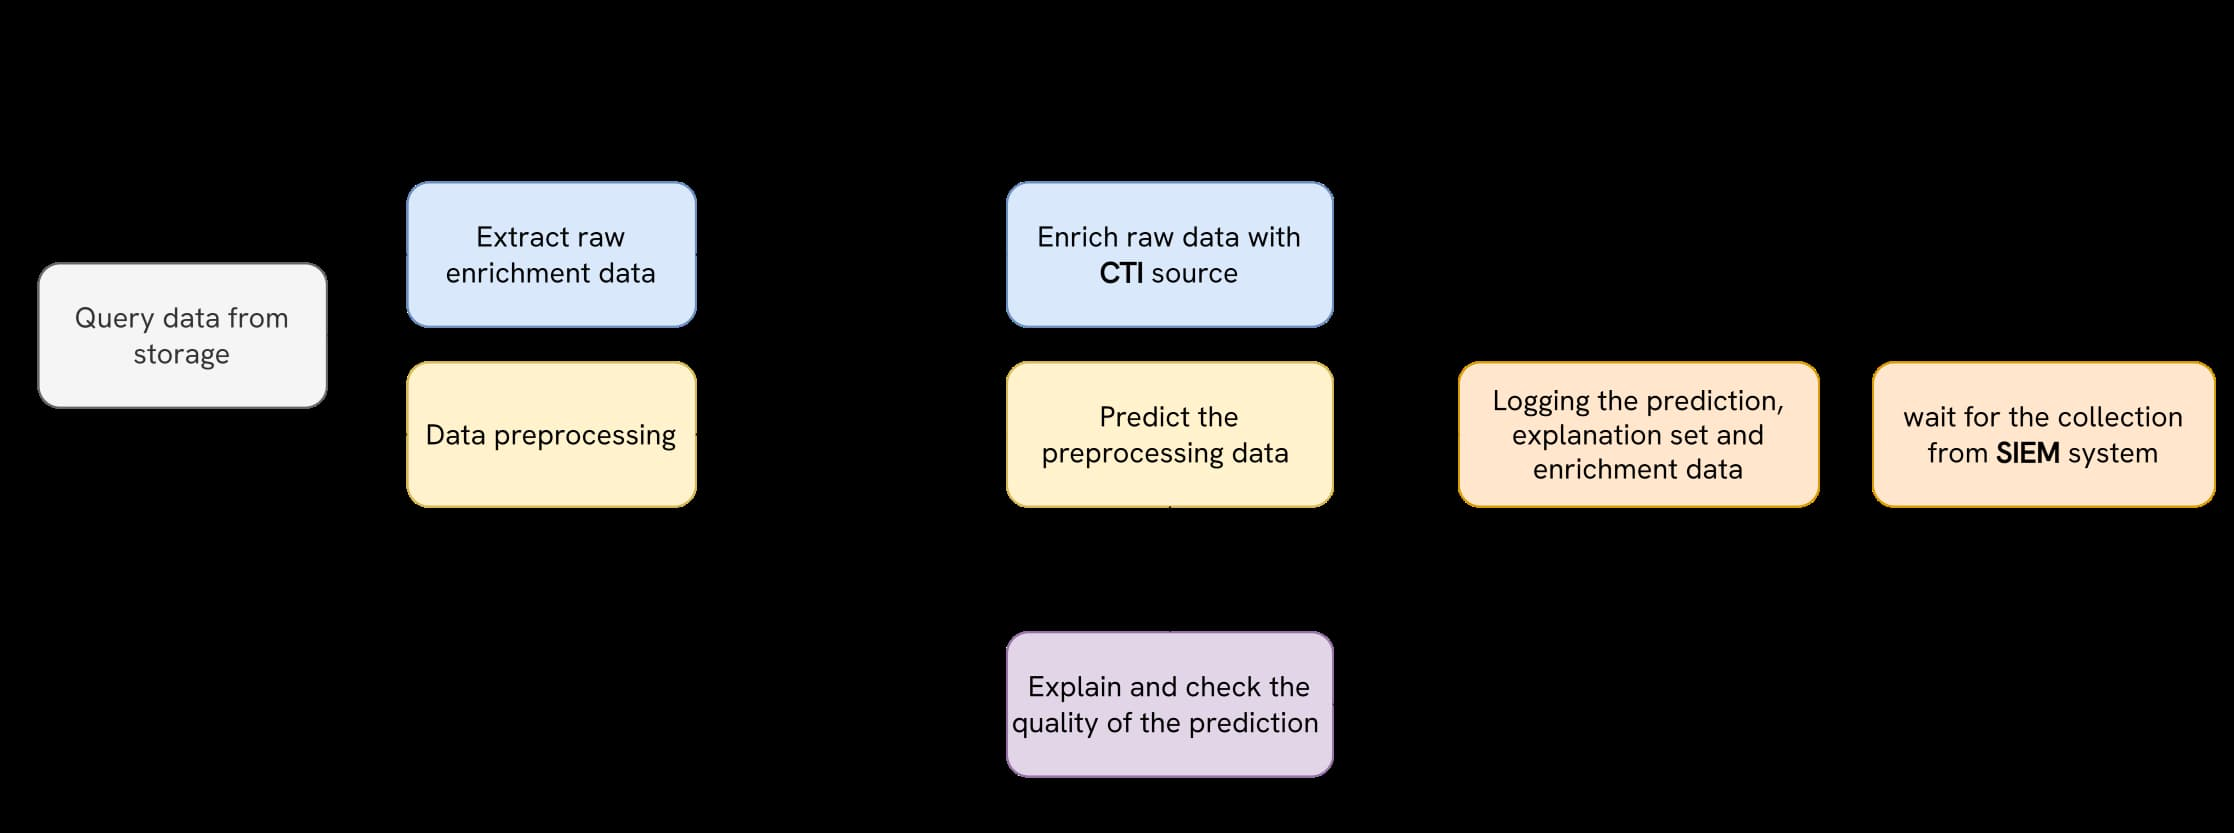
\includegraphics[width=\textwidth]{src/images/chapter3/preprocessing.jpg}
    \caption{Lưu đồ về cách thức hoạt động của hệ thống DPE}
    \label{fig:r&e-flowchart}
\end{figure}


\subsubsection{Luồng hoạt động chính}
Mặc dù dữ liệu được xử lý chia làm hai dạng là \textit{log} và \textit{flow}. Quá trình xử lý các dữ liệu của hệ thống PDE được đồng nhất và chia làm ba bước chính: trích xuất và tiền xử lý, làm giàu và cuối cùng là lưu trữ.

\begin{itemize}
    \item \textit{Trích xuất và tiền xử lý}: Dữ liệu được chuẩn hóa được truy xuất từ thiết bị lưu trữ của SIEM. Sau đó, đối với mỗi dữ liệu được truy xuất, hệ thống sẽ lọc các thuộc tính mà hệ thống IDS cần để dự đoán. Song song đó, hệ thống sẽ trích xuất các thông tin cần thiết cho quá trình làm giàu theo các tiêu chí trong \textbf{Mục \ref{sec:enrichment-criterion}} từ dữ liệu đầu vào.

    \item \textit{Làm giàu}: Dữ liệu làm giàu được chia làm hai dạng là dữ liệu làm giàu cục bộ và dữ liệu làm giàu từ bên ngoài. Song song với việc gửi các thuộc tính cần cho quá trình dự đoán đến và đợi các dự đoán trả về hệ thống IDS, hệ DPE sẽ gửi các thông tin cần cho quá trình làm giàu đến hệ thống CTI để thu được dữ liệu làm giàu từ bên ngoài. Bên cạnh đó, các dữ liệu đó sẽ được gửi đến hệ thống diễn giải dự đoán cũng như liên kết chúng với dữ liệu của tổ chức (liên kết IP với tên miền cục bộ, tên vùng mạng mà IP đó thuộc về, liên kết IP-PORT với dịch vụ đang chạy, ...) nhằm tạo ra các thông tin làm giàu cục bộ.

    \item \textit{Lưu trữ}: Cuối cùng, kết quả dự đoán từ hệ thống IDS và dữ liệu làm giàu được lưu trữ trong một tệp \textit{log} với một định dạng thống nhất và chờ được thu thập bởi hệ thống SIEM.
\end{itemize}

\subsubsection{Tiêu chí chọn thông tin cho quá trình làm giàu} \label{sec:enrichment-criterion}

%Tương tự như vấn đề đã đề cập ở phần \textbf{\ref{Chapter1}} về việc đầu ra của các hệ thống IDS sẵn có không phù hợp với các giải pháp săn tìm mối đe dọa, các thông tin làm giàu được trích xuất cũng phải phù hợp với các giải pháp săn tìm mối đe dọa. 
Dựa theo theo bài báo \cite{gunter2018practical}, các thông tin cần thiết cho quá trình săn tìm mối đe dọa cần đảm bảo phải trả lời được ít nhất một trong các câu hỏi sau: \textit{Mục tiêu được nhắm đến?}, \textit{Nơi cuộc tấn công bắt đầu?}, \textit{Thời gian cuộc tấn công diễn ra?}, \textit{Cuộc tấn công được diễn ra như thế nào?}, nên thông tin mà chúng ta trích xuất cũng phải có khả năng trả lời các câu hỏi trên hoặc có khả năng hỗ trợ quá trình làm giàu ở giai đoạn sau để có thể trả lời các câu hỏi đó. Ngoài ra, chúng ta cần đảm bảo các thông tin được trích xuất phải phù hợp với ngữ cảnh của từng dạng IDS. Ví dụ như chúng ta không thể sử dụng id của một tiến trình trên một điểm đầu để bổ sung thông tin cho quyết định của NIDS, cũng như sử dụng IP của một điểm đầu cuối mà điểm đó không tồn tại trong đồ thị gốc được phân tích bởi PIDS để bổ sung thông tin cho quyết định của PIDS đó.

\bigbreak\noindent
Dựa vào các câu hỏi ở trên chúng ta có thể thiết lập một tập hợp các thông tin có thể được chọn cho quá trình làm giàu có thể được chọn như bên sau:

\begin{itemize}
    \item \textit{Mục tiêu được nhắm đến?}: Chúng ta có thể suy luận ra được các điểm đầu cuối bị nhắm đến trong hệ thống dưới góc nhìn của NIDS thông qua IP nguồn-đích, port nguồn-đích, id của switch, ... Ngoài ra, trong trường hợp NIDS của chúng ta hoạt động ở chế độ phân loại, chúng ta cũng như đoán ra được hành vi mà kẻ tấn công thực hiện loại bất thường mà cuộc tấn công đó thuộc về (XSS, injection, DoS, scanning, ...). Bên cạnh đó, chúng ta suy luận ra mục tiêu cụ thể trên từng điểm đầu cuối thông qua mối quan hệ giữa các nút (các nút có thể là tệp tin, tiến trình, ...) được thể hiện thông quá thuộc tính của cạnh kết nối các nút đó (thuộc tính của cạnh có thể là thực thi, mở tệp tin, ghi tệp tin, kết nối đến một điểm nào đó, ...) trong đồ thị nguồn gốc được phân tích bởi PIDS.
    \item \textit{Nơi cuộc tấn công bắt đầu?}: Tường tự ở câu trên, chúng ta có thể trả lời câu hỏi này bằng thông tin về IP nguồn, IP đích, port nguồn, port đích, id của switch, ... hoặc id của các tiến trình, các tập tin, ... trên các điểm đầu cuối.
    \item \textit{Thời gian cuộc tấn công diễn ra?}: Có thể sử dụng thời gian mà cuộc tấn công bị phát hiện và thời gian khi mà luồng được tạo trên switch. Đối với PIDS, ta có thể sử dụng thời gian tệp tin, tiến trình được tạo, thực thi hoặc chỉnh sửa.
    \item \textit{Cuộc tấn công được diễn ra như thế nào?}: Đây là một câu hỏi rất khó để trả lời trong ngữ cảnh của NIDS. Tuy nhiên, với sự tham gia của PIDS chúng ta có thể phân tích cách cuộc tấn công diễn tra thông qua việc xâu chuỗi các sự kiện bất thường trong đồ thị gốc trên các điểm đầu cuối.
\end{itemize}

% \bigbreak\noindent


% \bigbreak\noindent


% \bigbreak\noindent


% \bigbreak\noindent


\bigbreak\noindent
Các thông tin nên được chọn cho quá trình làm giàu được tóm tắt như trong \textbf{Bảng \ref{tab:enrichment-criterion}} bên dưới.

\begin{table}[ht]
    \centering
    \caption{Tiêu chí chọn thông tin cho quá trình làm giàu}
    \label{tab:enrichment-criterion}
    \begin{adjustbox}{width=\textwidth}
    \begin{threeparttable}
    \begin{tabular}{|c|c|c|}
    \hline
    \textbf{Tiêu chí} & \textbf{NIDS} & \textbf{PIDS}\\
    \hline
    Mục tiêu được nhắm đến? & \makecell{IP nguồn-đích,\\port nguồn-đích, id của switch\\Loại tấn công\\(injection, DoS, scanning, ...)} & \makecell{Tương tác giữa các nút\\thông qua cạnh \\ (loại nút, loại cạnh)}  \\
    \hline
    \makecell{Nơi\\cuộc tấn công bắt đầu?} & \makecell{IP nguồn-đích,\\port nguồn-đích, id của switch} & \makecell{id của nút, IP của nút,\\id của tiến trình}\\
    \hline
    \makecell{Thời gian\\cuộc tấn công diễn ra?} & \makecell{Thời gian phát hiện tấn công,\\Thời gian \emph{flow được tạo trên switch}} & \makecell{Thời gian tạo, thực thi, \\  chỉnh sửa của tệp tin, \\ tiến trình} \\
    \hline
    \makecell{Cuộc tấn công được\\diễn ra như thế nào?} & - & \makecell{Chuỗi các nút và cạnh\\được dự đoán là bất thường\\(id của nút, loại nút,\\id của cạnh, loại cạnh)}\\
    \hline
    \end{tabular}
    \end{threeparttable}
    \end{adjustbox}
\end{table}
